\documentclass{report}
\usepackage[utf8]{inputenc}
\usepackage{xcolor}
\usepackage{url}
\usepackage[nottoc]{tocbibind}
\usepackage{graphicx}
\usepackage[bottom]{footmisc}
\usepackage{float}
\usepackage{caption}
\usepackage{subcaption}


\title{Project Document: Deep learning \\ Team : Encoders}
\author{Shiva Paudel\\
Shubham Bery\\
Puranjit Singh\\
Kantilata Thapa\\
}
\date{}

\begin{document}

\maketitle

\tableofcontents

\begin{abstract}
Deep learning is a rapidly growing field, expanding over variety of sectors. Vision-based machine learning techniques are being used in agriculture as well. In this work we are trying to explore two different deep learning methods which can be used in technical advancement of farming and fruit processing sector. At first, we presented how deep learning can be used to detect weeds in crop and second we explored the techniques that are being implemented to detect and classify fruits based on their rottenness. Then we selected the former idea as our final project that is use of deep learning to detect weeds in soybean crop. Two different deep learning based models were proposed for this problem. We identified a data set to train the model. As the data set was not big enough to train the model from scratch, both the models make use of transfer learning with fine tuning of base layers. For our first approach, we tried to implement residual layers based pre-trained model on ImageNet data set called as ResNet50. Till now, we are able to get 95\% weighted accuracy. But, this performance was not consistent as loss values changed drastically because the model showed some signs of overfitting. We implemented a variation of ResNet50 architecture that makes use of Inception blocks to make the network wider and overcome the overfitting problem. Till now, we managed to achieve a validation accuracy of more than 98 \% with not so varying loss against epochs graph.
\end{abstract}

\chapter{Milestone 1: Project Ideas}

\section{Introduction}
Agriculture is the life-sustaining element for many people around the globe. But agriculture itself faces numerous challenges in terms of biological, ecological and developmental aspects. People from both developing and developed countries are facing the challenges in their own terms regarding the production and consumption of agriculture commodities. On the other hand, production and consumption of agricultural products needs to be balanced side by side to feed the burgeoning population along with food safety measures. Among the numerous problems encountered so far, encroachment of major crop fields by weeds is the one, causing decline in yield and quality of crop products. Similarly, consumption of healthy and fresh fruits is must for the rapid advancement of human race and to boost immune system. Global agriculture demands more scientific study yet practical solutions to successfully combat the pressing challenges. Therefore, deep learning techniques come in frontier to deal with such challenges with promising results and large potentials with the use of large image datasets for image identification as well as classification approaches. This project deals with two different problems in agriculture world with different approaches of Convolution Neural Networks (CNNs).  
\iffalse
\begin{figure}
    \centering
    \includegraphics[width=\textwidth]{figs/ai-and-compute-all-2.png}
    \caption{Compute for cutting-edge deep learning projects vs.\ time (source:~\cite{AI-compute18}).}
    \label{fig:compute}
\end{figure}

\begin{table}[]
    \centering \caption{Top-5 error on ImageNet for various convolutional architectures.}
    \begin{tabular}{|c|c|c|} \hline
      Architecture   &  Year & Top-5 Error \\ \hline
    AlexNet & 2012     & 17\% \\
    GoogLeNet & 2014 & 7\% \\
    ResNet & 2015 & 3.6\% \\ \hline
    \end{tabular}
 
    \label{tab:CNN-perf}
\end{table}
\fi
\section{Project Idea 1: Weed detection using Deep Learning }
\subsection{Problem}
In the USA, weeds cost about approximately 33 billion USD in  crop production annually \cite{4}. Maize is the third most important staple cereal crop after Rice and wheat but yield loss in maize is estimated about 25 percent due to several types of weeds \cite{2}. Additionally, weeds harbor various insects and pests that are very harmful to the main crop. Similarly, in many developing countries hand weeding is being replaced by herbicide use due to labor shortage and in developed countries there is already high dependency on herbicide for weed control. But over reliance on herbicide has resulted in many unique herbicide-resistant weeds which are even more difficult to control. Therefore, the application of deep learning and modeling approaches can be a solution to achieve site -specific and economical weed management for long term in maize crop.
 Weed management is one of the most important crop production practices. Global increase in herbicide use to control weeds has led to issues such as evolution of herbicide-resistant weeds, off-target herbicide movement, etc. Precision agriculture advocates site-specific herbicide application to achieve precise and right amount of herbicide spray and reduce off-target herbicide movement. Recent advancements in Deep Learning have opened possibilities for adaptive and accurate weed recognition for field based site-specific herbicide applications with traditional and emerging spraying equipment \cite{1}.\par
Due to identical spectral signature of weeds and host plants, spectral features are insufficient to distinguish between the two. 

\subsection{Application}
With machine vision system we can leverage upon their easy to modify and implement advantage to
 develop site specific weed management strategies. A weed map of a specific site can be created. This method can be a huge steppingstone toward autonomous picking of weed and utilization of remote sensing techniques in farming. With the use of proper sensors, this method can further be advanced to in field weed density evaluation and precise positioning of weed.  Currently, variety of unmanned aerial vehicles (UAVs) are being used in precision agriculture with limited applicability, with introduction of proper weed detection techniques UAVs scope can be stretch into weed management as well. Another big issue is that farmers are using immense number of herbicides to eradicate the unwanted weed, the herbicides affect the crop itself and might lead to health-related problem on consumer. This vision-based weed detection technique will also be very fruitful to lower the herbicide use.
\iffalse
\begin{itemize}
    \item site -specific weed management strategy can be developed.
    \item Weed map can be created and weed detection can be done using remote sensing applications.
    \item Weed density evaluation in field can be done and precise positioning of weed can be detected for site-specific management.
    \item Use of precision agriculture techniques in handling and controlling the spraying of herbicides in the fields 
    \item Variable rate herbicide spraying
\end{itemize}
\fi
\subsection{Approaches}
Initially our thoughts were to collect our own dataset, but with suggestion from Dr. Scott We have identified a dataset with 15000 labelled images from internet(). We will identify some object detection algorithm and use the dataset for fine tuning the model. Figure \ref{fig:process} shows the workflow of project.\par 
\iffalse
High-resolution image data will be collected using UAV (Unmanned Aerial Vehicles). We will label the images with pixel wise segmentation to annotate the weed. With labelled images we will train object detection models to identify the weeds. Figure \ref{fig:process} shows the workflow of project.\par 
\fi
\begin{figure}[h]
    \centering
    \includegraphics[width=\textwidth ]{figs/workflow1.jpeg}
    \caption{ Proposed workflow}
    \label{fig:process}
\end{figure}
\newpage
\section{Project Idea 2: CNN-based rotten fruit identification}
\subsection{Problem}
One of the most important challenge faced by today's fruit harvesters is properly identifying and isolating the rotten fruit from fresh fruit.  Failing to remove rotten fruit in early stage of rottenness usually lead to large economic loss as the rottenness is highly infectious.  Classifying rotten fruit is fundamental for higher productivity and long life of the fruit. Typically classification of fruit is done manually, and is a laboursome, expensive, and time-consuming task. Human efficiency in doing such types of repetitive tasks is usually very low. There is a need of automatic system which can classify the fruit based on rottenness. \par
 In the past, several techniques have been tried to detect rottenness of the fruit such as X-ray classification, thermal imaging, impedance etc. \cite{rotten1}. These techniques are hazardous to fruit itself as well as to the human performing the test. With introduction of computer vision and deep learning several classification task are being done with trained automatic machine \cite{rotten2}. And use of machine vision to detect rottenness of a fruit could be a harmless and efficient way. In recent time people are starting to use several CNN based technique to classify the rotten fruit \cite{rotten3}. Here in this project we are trying to implement a deep learning model to classify the rotten fruits from the fresh ones.\par
 \subsection{Application}
 This deep learning based method of identifying fruit and classifying them into two group based on their rottenness will be very useful to separate the rotten fruit from those are good to use. detecting fruit might not be very useful for harvesters but classifying them into two group based on rottenness will cut off their most expensive and tiresome manual work. This method is useful itself, but we can confidently say that the most important application will be the further techniques in automation that this method brings into picture. Although, due to the resources and time constrain we are developing the method to classify only three types of fruit, this idea can be further expanded to classify other fruits with little effort.
 \iffalse
 \begin{itemize}
    \item will be applicable to detect rotten fruit
    \item will be helpful for further automation in fruit processing
    \item can be extended to classify many type of fruit
\end{itemize}
\fi
 \subsection{Approaches}
 In this project we will train a model to classify three different fruits that are Tomato, Avocado, and Oranges into six categories:
 \begin{itemize}
     \item Fresh Apple
     \item Fresh Oranges
     \item Fresh Banana
     \item Rotten Apple
     \item Rotten Oranges
     \item Rotten Banana
 \end{itemize}
 We will use ResNet50 model as a base model for our transfer learning. To identify the fruit we will use kaggle fruit 360 datasets where they have 90438 images divided into 131 fruit and vegetable categories. Initially our thoughts were to collect our own dataset for rotten fruit identification, but with suggestion from Dr. Scott We now have identified labelled dataset available at Kaggle website for categorical classification of rotten and fresh fruits. Following Figure \ref{fig:pro} shows a basic idea of the model.
\begin{figure}[h]
    \centering
    \includegraphics[width=0.9\textwidth ]{figs/flow.drawio.png}
    \caption{Basic Model Scamatic}
    \label{fig:pro}
\end{figure}


\section{Conclusions}

Proper automation in agriculture using deep learning approaches can be used to increase substantial yield and decrease economic loss either by controlling weed or by identifying the rotten fruit. Similarly, image processing is a non-invasive and effective tool that can be applied to detect and identify the on the farm and storehouse and effectively remove them . Application of image processing algorithms helps to identify weeds by shape, color, texture, and size features. Since hand labor is getting expensive day by day using automatic detection and classifying technology might lead to a great economic growth. 
\iffalse
\textcolor{red}{Remember to cite sources using BiBTeX and add those references to the end of this document!}

It is okay to cite some websites and tutorials (if you first look up how to properly cite them!), but you must also cite some refereed publications from conferences and/or journals.

Sample citation

Finally, in Table~\ref{tab:contribution1}, list each member of your team with a brief summary of that member's contribution to this milestone.

\begin{table}[h]
    \caption{Contributions by team member for Milestone~1.}
    \centering
    \begin{tabular}{|c|c|} \hline
    {\bf Team Member}     &  {\bf Contribution}  \\ \hline
    Shubham Berry     &  Contribution1 \\
    Shiva Paudel    &  Contribution2 \\
    Kantilata Thapa     &  Contribution3 \\ 
    Puranjit Singh     &  Contribution3 \\ \hline
    \end{tabular}
    \label{tab:contribution1}
\end{table}
\fi

\chapter{Milestone 2: Project Selection}
\iffalse
In this chapter, you should select your project, formally define it, and propose two approaches, each with a work plan.  You should follow the The Heilmeier Catechism, which is a set of questions used to evaluate proposed research programs:  
\begin{enumerate}
    \item What are you trying to do? Articulate your objectives using absolutely no jargon.
   \item How is it done today, and what are the limits of current practice?
   \item What is new in your approach and why do you think it will be successful?
   \item Who cares? If you are successful, what difference will it make?
   \item What are the risks?
   \item How much will it cost?
   \item How long will it take?
   \item What are the mid-term and final ``exams'' to check for success?
\end{enumerate}

Also, remember to update your abstract when you've completed this chapter. 
\fi

\section{Introduction}
We will be going forward with our first project idea of using deep learning techniques to detect weeds in agricultural fields. There were two main reasons that inspired us to work on this project. First, this work is much related to our area of research in which all of us would be working on using advanced image processing techniques and deep learning methods later in our research work. Second, recent advancements and interesting applications of convolutional neural networks in object detection field have motivated us to learn their application too. We will make use of convolution neural networks and transfer learning approach to build deep learning model for our final project. 

\subsection{Problem Definition}
The main goal of this project is to build a robust model that is able to detect weeds in agricultural fields. This model development has an array of use cases that would help in managing and increasing crop production to the farmers in multiple ways. The main advantages to develop a model like this would be to implement variable rate spraying of herbicides in the fields, that would prevent herbicide spray in unwanted areas and this could also help in increasing crop production. We have gathered an online dataset including images of soil, crops and weeds that we will use to build our model. The two different approaches that we would be using for developing our models involve use of inception and ResNet networks in collaboration with transfer learning.

\subsection{Motivation and Applications}
The strong motivation behind this project first started with the growing application of computer vision techniques in agriculture that allows efficient and precise farming with less human labor. Weed detection in agricultural fields is a very challenging task. The main obstacles that one faces during training a deep learning model to detect weeds are color, texture and shape similarity of weeds with the crop. Some other problems associated with weed detection includes occlusion of crops and weeds, shadow effects in natural weed image, effects of illumination conditions, different species of weeds at different growth stages and motion blur and noise effects during capturing image \cite{hasan2021survey}. Deep learning methods we will use during this project can be a base to successfully detect weeds considering human labor, time, and environmental impacts caused by the application of herbicides.\par
Also, they can be further modified to develop site-specific weed management strategies, weed density evaluation and the precise positioning of weeds in fields. Overall, these methods propose huge possibilities and solutions for reducing production cost, management cost, and protecting the environment by minimizing the traditional techniques of herbicide spraying over the whole field.

\section{Dataset}
Dataset being used has a set of UAV captured images, all those with occurrence of weeds were selected. These images were segmented and annotated with their respective class. The image dataset has a total of 15336 segments, being 3249 of soil, 7376 of soybean, 3520 grass and 1191 of broadleaf weeds \cite{kaggle}.Each dataset has pixel size of around $200\times180$. We will use train to test ratio of 80:20. The loss function and the evaluation metric will be the mean squared error. Figure \ref{fig:lebeled_im} shows the four different types of images in datasets.

\begin{figure}[H]
\centering
    \begin{subfigure}[b]{0.3\textwidth}
         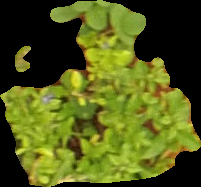
\includegraphics[width=\textwidth]{Broadleaf.png}
         \caption{Broadleaf}
         \label{fig:1}
     \end{subfigure}
    
     \begin{subfigure}[b]{0.3\textwidth}
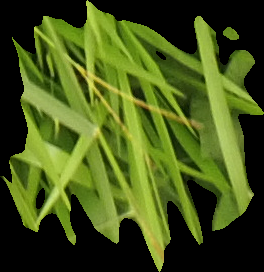
\includegraphics[width=\textwidth]{Grass.png}
         \caption{Grass}
         \label{fig:2}
     \end{subfigure}
     \begin{subfigure}[b]{0.3\textwidth}
         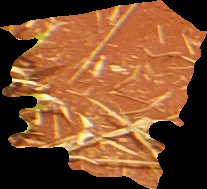
\includegraphics[width=\textwidth]{Soil.png}
         \caption{Soil}
         \label{fig:3}
     \end{subfigure}
     \begin{subfigure}[b]{0.3\textwidth}
         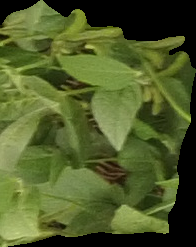
\includegraphics[width=\textwidth]{Soyabean.png}
         \caption{Soybean}
         \label{fig:4}
     \end{subfigure}
     \caption{Four different categories of images in datasets}
    \label{fig:lebeled_img}
\end{figure}
\section{Resources Required}
In order to analyze the available datasets proposed for this project work, we plan to utilize the resources that are available on crane. We plan to use Keras API for training, testing, and evaluating. 

\section{Proposed Method 1: Weed detection using Inception models}

Transfer learning means to take features learned on one problem, and leveraging them on a new problem. The first method uses a pre-trained model called Inception. This architecture includes inception modules, that combines pooling layers with filters of various sizes, allowing them to utilize the benefit of each filter size, for example, wide filters ($5 \times 5$) are able to extract main information, whereas small filters ($1 \times 1$) can extract local information \cite{szegedy2016rethinking}. This configuration can help the model to differentiate between plant leaves and weeds.


\begin{figure}[h]
    \centering
    \includegraphics[width=\textwidth]{figs/inceptionv3.png}
    \caption{Inception V3 Model \cite{szegedy2016rethinking}}
    \label{fig:compute}
\end{figure}

The following steps will be taken to implement our first approach:
\begin{enumerate}
	\item Transform and split the images into training and testing set  from dataset to feed into the model. 
	\item Download the pre-trained weights for the model.
	\item Freeze weights to avoid deleting any of the information they contain during further training rounds.  
	\item Fine tune model to add new layers to the architecture to solve the potential problems of overfitting, low learning rates etc, so that it detects weeds better.

\end{enumerate}
\begin{figure}[h]
    \centering
    \subfloat{{\includegraphics[width=0.4\textwidth]{figs/sparse.png} }}%
    \qquad
    \subfloat{{\includegraphics[width=0.2\textwidth]{figs/Densely.png} }}%
    \caption{Sparsely connected model vs Densely connected model}%
    \label{fig:Arch1_Tr3}%
\end{figure}

Common problem faced while creating deeper models are overfitting the training set and increased computational resources. Inception tries to solve these with the use of sparsely connected network architectures that will replace fully connected network architectures, especially inside convolutional layers. Thus in the inception model instead of having deep layers, we have parallel layers making the model wider rather than making it deeper. We plan to fine tune and implement this method by the first week of March.


\section{Proposed Method 2: Weed detection using Residual Architecture}

In the second approach, we are basically interested to construct a deep learning model using Residual networks. During a literature review for the topic \cite{ResNetArchi}, we came to know that residual layers could be used to construct Neural networks, involving deeper layers and skip connections that help to overcome the problem of vanishing gradient descent during the training phase. Predicting weed locations in a soybean fields is a cumbersome task and would require extensive training of deep neural networks to detect weeds in the fields with high precision and recall outputs from the results. We would use transfer learning techniques and make use of a pre-trained model already trained on ImageNet dataset with a ResNet50 architecture as a second approach towards our final goal of weed detection in agricultural fields which would help us to develop more robust models that could perform better as compared to former. The following steps will be taken to implement our first approach:

\begin{enumerate}
	\item Splitting the original dataset into two separate categories : train and test. The training of our model would be performed on the training dataset and checking on how well our model is generalising is performed on the testing dataset. 
	\item Loading the pre-trained weights for ResNet50 model already trained on ImageNet dataset from the Tensorflow Keras API
	\item The pre-trained network is used to extract features and train the network to detect different categories of objects inserted into the model for training 
	\item Fine tune model to add new layers to the architecture to solve the potential problems of overfitting, low learning rates etc, so that it detects weeds better.

\end{enumerate}
\begin{figure}[H]
\centering
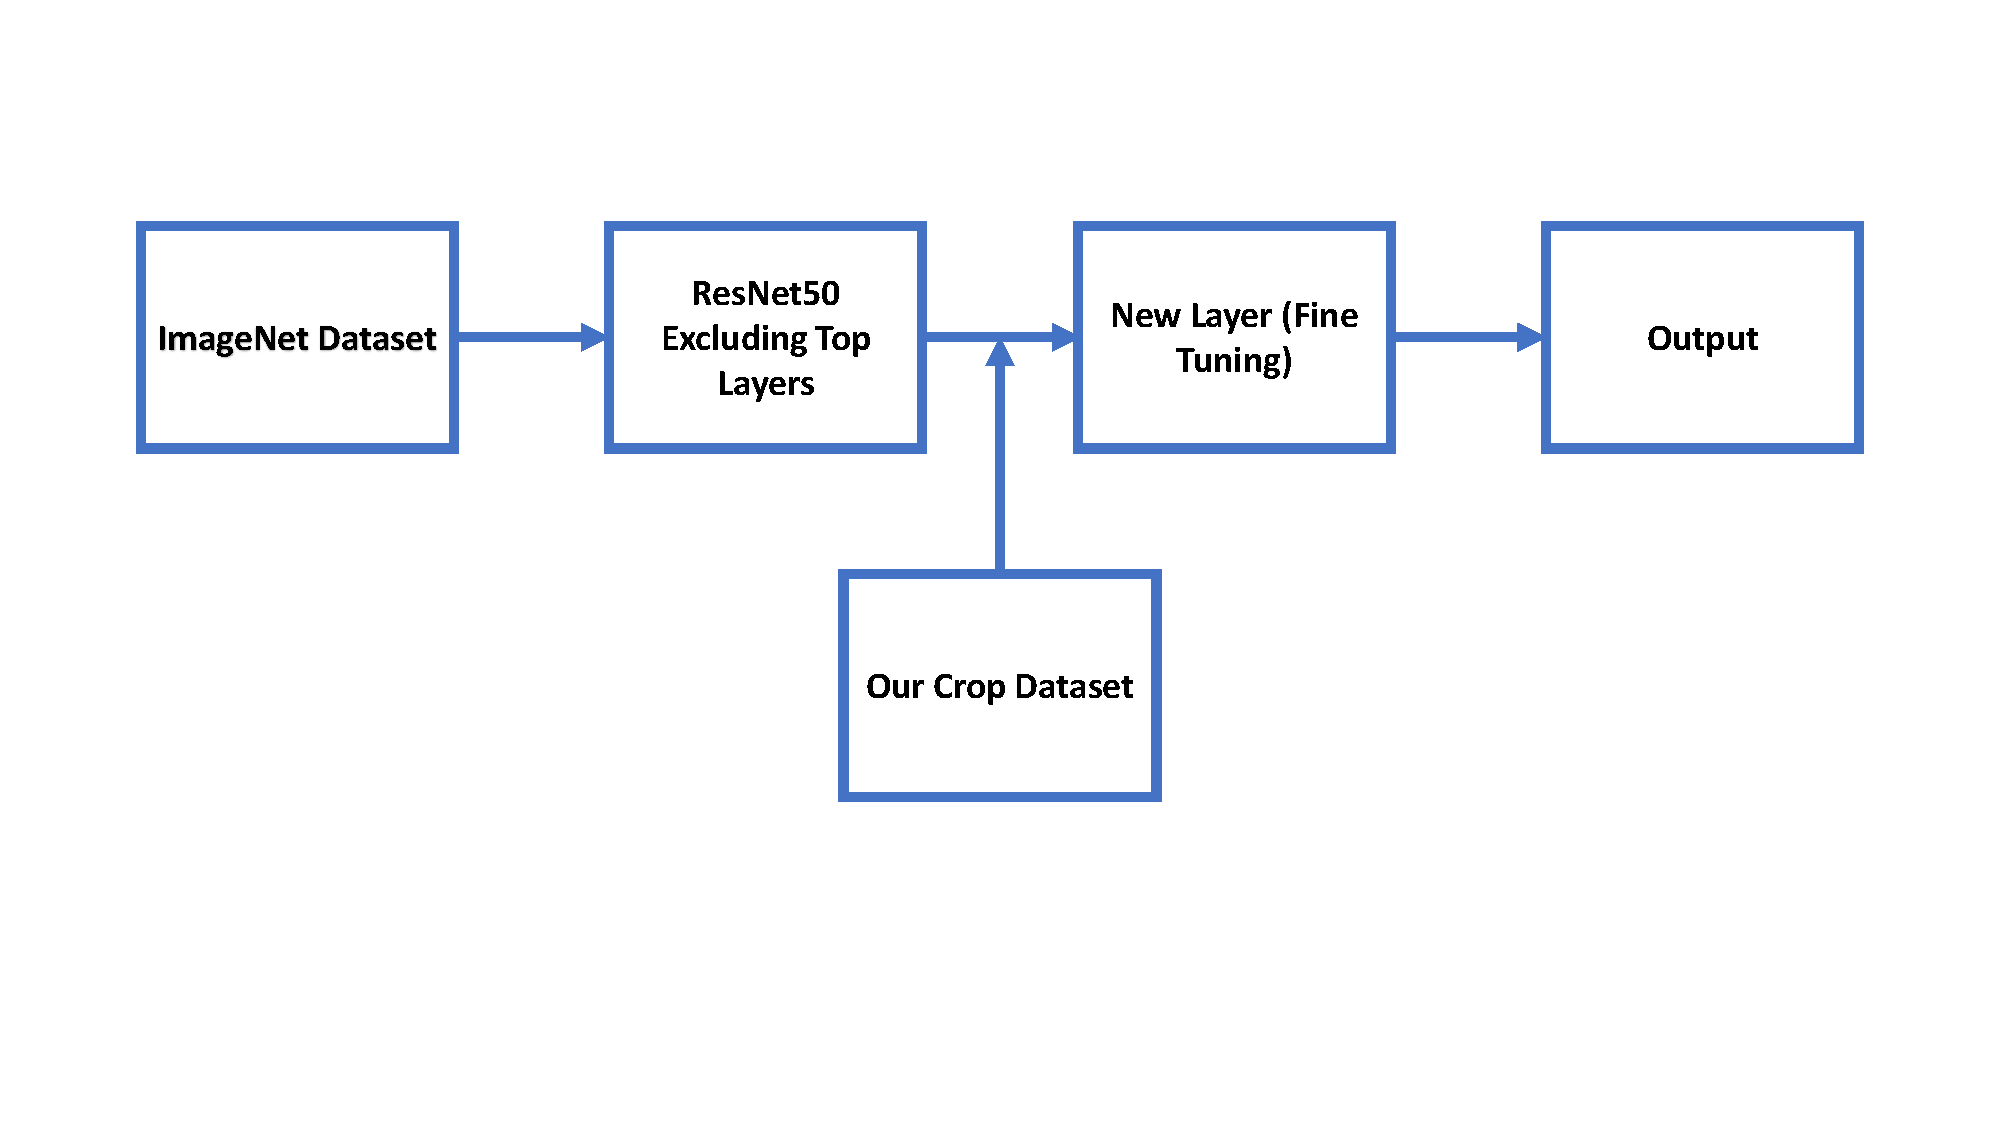
\includegraphics[width=\textwidth]{pic1.pdf}
\caption{Flowchart}
\label{fig:Flowchart}
\end{figure}

The main intuition behind using residual layers in training of our weed detection model is the presence of ($1 \times 1$) convolutional layers in them. These ($1 \times 1$) convolutional layers help the model in detecting even small features in an image. On comparison with other things like crops, grass that share quite resemblance with each other, it sometimes becomes difficult to detect difference between them from a naked eye. Using residual block with lower convolutional filters helps the model in detecting small feature sets of weeds and help in developing more robust models. The difference between a residual block and a set of normal convolutional filters in a neural network could be understood from Figure \ref{fig:ResidualBlock}. 

\begin{figure}[H]
    \centering
    \includegraphics[width=\textwidth]{ResNetBlock.png}
    \caption{Residual block }
    \label{fig:ResidualBlock}
\end{figure}


\begin{figure}[H]
    \centering
    \includegraphics[width=\textwidth]{ResNet50.jpg}
    \caption{ResNet50 Architecture}
    \label{fig:ResNet50}
\end{figure}

We will use ResNet50 architecture in our second approach to work over our weed detection problem in our deep learning project. We will start working on this approach after we obtain the results for our first model i.e. right after our spring break.


\section{Conclusions}

We have decided to choose the weed detection project with little changes in the previously proposed objective. We have now figured out the datasets with labeled images for training and testing datasets. Here in milestone 2, we have proposed two methods for detecting weed in soybean crops. Firstly, we are proposing a method where we will build a transfer learning model based on the inception method. The inception method is supposed to be fast and can be useful for real-time weed detection. Secondly, we are proposing a similar model to detect weed but with ResNet50 which is slower but more efficient as compared to the former. If we get enough time and computational we also might want to train our dataset on both the models and compare them for execution time and efficiency trade-off.

\begin{table}[h]
    \caption{Contributions by team member for Milestone~1.}
    \centering
    \begin{tabular}{|c|c|} \hline
    {\bf Team Member}     &  {\bf Contribution}  \\ \hline
    Shubham Bery     & Method Description \\
    Shiva Paudel    & Documentation\\
    Puranjit Singh     & Concept and Idea Formulation \\
    Kantilata Thapa     & Documentation \\ \hline
    \end{tabular}
    \label{tab:contribution1}
\end{table}

\chapter{Milestone 3: Progress Report 1}

\section{Introduction}
As proposed in the last milestone, we are working on our weed detection model using deep learning techniques. Our aim is to develop a convolutional neural network (CNN) using transfer learning technique that can detect weeds in an input image of field. For this milestone, we tried implementing one of the proposed approaches that makes use of residual networks to construct the deep learning model. The reason behind using this architecture is the presence of (1 × 1) convolutional layers in it which help the model to detect even the slightest significant features in an image. This enables the model to see the minute differences between the main crop and similar looking unwanted growth. Residual layers are helpful in developing neural networks, involving deeper layers as it skips connections between layers to address the problem of overfitting and vanishing gradient during the training phase. As the dataset used for training was comparatively smaller, we had to use data augmentation techniques that generated different versions of the existing dataset artificially to increase its size. To speed up the training process, we are making use of transfer learning techniques. We used a model that is based on ResNet50 architecture pretrained on the ImageNet dataset.  To best fit the model to the dataset at hand, we also fine-tuned the weights of existing layers in the base architecture. Furthermore, we implemented early stopping not to overfit the model by training it for a longer duration. With this architecture, we noticed some large fluctuation in loss value indicating a poor fit. We tried fine tuning the model which made the significant improvement in performance. We plan to implement InceptionResNetV2 architecture along with hyper-parameter optimization in our future runs.  
\label{sec:M3-intro}


\section{Experimental Setup}
To complete this project, labeled image dataset with 15336 labeled images were downloaded from Kaggle \cite{kaggle}. Further information on how and where the images were collected is not disclosed by the authors. To increase the size of the training dataset we used the data augmentation technique. We used the techniques such as rotating, shifting, and flipping of the images using existing techniques available in keras for data augmentation. We used the updated dataset including images from data augmentation to train a convolution neural network for a classification task. We decided to implement the ResNet50 model with an additional dense layer with 4 neurons with softmax activation function for categorical classification. To compile the model, we used ‘adam’ as the optimizer, ‘categorical cross entropy’ loss function as an accuracy metric. The model was trained with the augmented images as input and corresponding label as target. We used Crane, a powerful computing machine at our disposal during the course to train the model.

\subsection{Datasets}
The ‘Weed Detection in Soybean Crop’ dataset contains a total of 15336 segmented images, being 3249 of soil, 7376 of soybean, 3520 grass and 1191 of broadleaf category of weeds. Each image in the dataset has a pixel size of around 200x180. We split the dataset into 8:2 training and testing images. We use augmentation techniques to increase variability as well as the number of images. For data augmentation we used already available method in Keras namely ImageDataGenerator with a batch size of 32 and randomly shifted, flipped, and scaled the images to increase our existing dataset.

\subsection{Architecture}
The model architecture we used for the weed detection problem in a soyabean crops is ResNet50. We used this architecture because it allows us to train ultra-deep neural network with hundreds or thousands of layers and still can achieve higher accuracy. Also, ResNet50 architecture can be used to construct Neural networks, involving deeper layers and skip connections that help to overcome the problem of vanishing gradient descent during the training phase. We used transfer learning techniques and used a pre-trained model already trained on ImageNet datasets. This dataset was split into training and testing set. The training was performed on training dataset and the model performance was observed on testing dataset. ResNet50 model already has pre-trained weights which were uploaded and used in our code from TensorFlow Keras API. This pre-trained network extract the features and train the network to detect four categories of objects inserted into a model. Our approach is to fit the model firstly freezing the existing weights and then fine tuning the exisitng weights which were automatically done based on the demand for our dataset. We have added one dense layer with 4 neurons for four categorical classification of the intended identification. The figure
\ref{fig:Flowchart} summarizes our approach on training the model.
\begin{figure}[H]
\centering
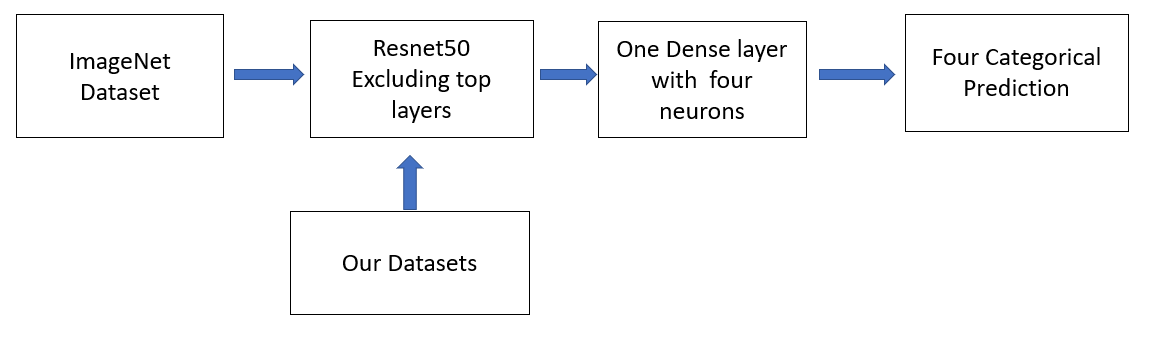
\includegraphics[width=\textwidth]{35.PNG}
\caption{Flowchart}
\label{fig:Flowchart}
\end{figure}

\subsection{Performance Measures}
The four categories labels were converted to one hot vector and probabilistic categorical cross entropy is used as our performance metric. The categorical cross entropy loss computes the loss between true and predicted labels. We implemented early stopping to limit training of our model at an appropriate time by monitoring the improvement in the validation loss metric. 

\subsection{Hyper-parameter}
As we have decided to fine tune ResNet50 architecture. The predefined model architecture has limited our ability to try different sets of hyper-parameters. For the first progress report we have decided to run our model with early stopping callbacks of 5 epochs patience for 10 epochs. Even though we were bound to limited sets of hyper-parameters for tuning we still have power over the number of neurons on additional layers and the dropout percentage in subsequent layers. In our future runs we plan to add a few more fully connected dense layers with a dropout layer in between. Along with additional layers, we will also be seeking other logical ways of hyper-parameter optimization. 



\section{Experimental Results}
We fitted our model as described in the previous section. We froze all the layers except the initial input layer, we added one dense layer with 4 neurons to categorically classify the four distinct categories. With the weight frozen we achieve a training loss as low as 0.6 and validation loss as low as 0.62. The following figure \ref{fig:Frozen} shows the learning curve of the fitted model. The validation curve clearly shows the sign of a poorly fitted model as it is fluctuating over large loss value. With this performance, we hypothesize that unfreezing all the layers of ResNet50 and fine tuning the weights with our dataset might lead to a better performance. 

\begin{figure}[H]
\centering
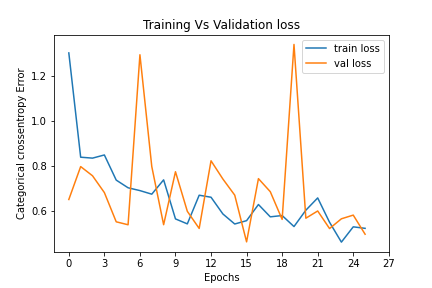
\includegraphics[width=\textwidth]{LossVal_lossR50Freeze.png}
\caption{Learning Curve for ResNet50 with weight frozen}
\label{fig:Frozen}
\end{figure}

The figure \ref{fig:Fine-Tuned} shows the learning curve for the fine-tuned fitting approach. With fine tuning we achieve a final loss of below 0.4 for both training and validation dataset with little fluctuation in validation loss.  In our next progress report, initially we will seek a way to optimize the hyper-parameters. The results from optimized model will be compared with the performance of the current model. The ResNet50 architecture had approximately 23 million trainable parameters. As we have discussed in milestone 2 there are other architecture which might perform better than using ResNet50. We are reviewing some literature to identify a better approach to obtain much better result. We also plan to implement InceptionResNetV2  model for transfer learning. However, the trainable parameters in both ResNet50 and InceptionResNetV2 are equal, the wider approach of InceptionResNetV2  model might lead to better classification.
\begin{figure}[H]
    \centering
    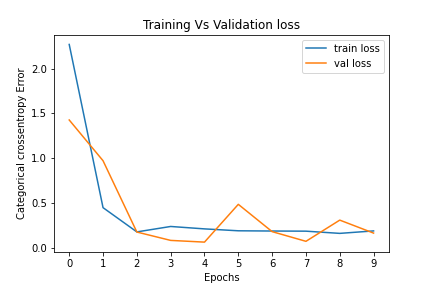
\includegraphics[width=\textwidth]{LossVal_lossR50FineTune.png}
    \caption{Learning Curve for ResNet50 fine-tuned}
    \label{fig:Fine-Tuned}
\end{figure}




\hfill

\begin{tabular}[H]{ | p{3cm}||p{2cm}||p{2cm}||p{2cm}||p{2cm}|}
\hline
 \multicolumn{5}{|c|}{ Table 3.1 :Metrics }\\
 \hline
 Serial Number & Precision & Recall & F1-Score & Support\\
 \hline
 0 - Grass & 0.93 & 0.89 & 0.91 & 350 \\
 1 - Soil & 0.98 & 1.00 & 0.99 & 324\\
 2 - Soybean & 0.97 & 0.99 & 0.98 & 733\\
 3 - Weeds & 0.78 & 0.76 & 0.77 & 120 \\
 Accuracy &  &  & 0.95 & 1527\\
 Macro Average & 0.92 & 0.91 & 0.91 & 1527\\
 Weighted Average & 0.95 & 0.95 & 0.95 & 1527\\
 \hline

\end{tabular}

\begin{figure}[H]
\centering
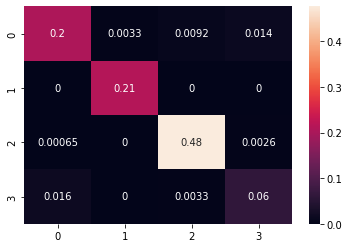
\includegraphics[width=\textwidth]{Confusion_matrix.png}
\caption{Confusion Matrix True vs Predicted}
\label{fig:CM}
\end{figure}



\section{Discussion}

Reviewing the literature, use of residual networks was a step taken in the right direction. However, the results we got were not aligned to what we thought \cite{theckedath2020detecting}. We initially froze the base network weights and quickly found that it was a dead-end with no gradual improvement in the model performance as both the training and validation losses were significantly higher. After this, we fine-tuned the model along with unfreezing the weights of base layers, we witnessed an improvement over the first trial. Still, we believe that the hyper-parameters can further be tuned to get a better performance out of this architecture. However, fine-tuning comes at a significant computation cost and a higher risk for overfitting to the training data. So, sufficient measures will be needed to mitigate this overfitting problem such as the use of dropout layers. In our future work we will work towards reducing the overfitting of this model along with implementation of our second proposed architecture, InceptionResNetV2 . The main intuition behind using transfer learning techniques using weights already trained on InceptionResNetV2  architecture is because these are wider networks as compared to ResNet architectures and could help us to learn and perform better on training the model and therefore getting good results for further classification tasks.

\section{Conclusion}

Till now, we observed that transfer training is one of the right approaches that we could use to train a deep learning model with a smaller dataset. We used a pretrained ResNet50 model already trained on ImageNet dataset for our project. All the results, such as the learning curves, showed some benefit of fine-tuning but the results were not promising as expected. We could not perform ample hyper-parameter tuning in the work so far but expect that our findings will get better with the right set of hyper-parameters. For the next milestone, we also plan to implement a different architecture InceptionResnetV2 and will try to compare the results with further fine-tuned ResNet50.


\begin{table}[H]
    \caption{Contributions by team member for Milestone~1.}
    \centering
    \begin{tabular}{|c|c|} \hline
    {\bf Team Member}     &  {\bf Contribution}  \\ \hline
    Shubham Bery     & Writing the report \\
    Shiva Paudel    & Writing the report and helping on final model development\\
    Puranjit Singh     & Writing the code and running the entire model\\
    Kantilata Thapa     & Writing and finalizing the report\\ \hline
    \end{tabular}
    \label{tab:contribution1}
\end{table}


\chapter{Milestone 4: Progress Report 2}


\section{Introduction}

Our project aims to develop a model that can detect weeds in soyabean crops using deep learning techniques. The method involves developing a supervised learning model based on convolutional neural network (CNN) making use of transfer learning that can classify weeds in an input image. In the last milestone, we tried implementing one of the proposed approaches that made use of ResNet50 pretrained model to build a deep learning model. But the model did not work as expected and showed inconsistent performance. After fine-tuning the model and unfreezing the weights, loss curve showed some consistency and improvement over the previous trials. We wanted to try out a different architecture so that the performance can be improved. After reviewing the literature, we found that using residual connections along with inception blocks can lead to an even better performance \cite{szegedy2017inception}. InceptionResNetV2 is a convolutional neural network that is trained on more than a million images from the ImageNet database. The network is 164 layers deep and can classify images into 1000 object categories. So, we went ahead and used a pretrained instance of InceptionResNetV2. As the dataset used for training was comparatively smaller, we had to use data augmentation techniques that generated different versions of the existing dataset artificially to increase its size. We witnessed a significant improvement in model’s performance with validation accuracy of more than  98\%.


\section{Experimental Setup}
For this project, labeled image dataset with 15336 labeled images were downloaded from Kaggle \cite{kaggle}. To increase the size of the training dataset we used the data augmentation technique. We used techniques such as rotating, shifting, and flipping of the images using existing techniques available in keras for data augmentation. Further information on how and where the images were collected is not disclosed by the authors. We used the updated dataset including images from data augmentation to train a convolution neural network for a classification task. For this time, we decided to implement InceptionResnetV2 Model with dense layer and SoftMax activation function for categorical classification. To compile the model, we used ‘Adam’ as the optimizer, ‘categorical cross entropy’ loss function as an accuracy metric. The model was trained with augmented images as input and corresponding label as target. We used Crane, a powerful computing machine at our disposal during the course to train the model. The following figure summaries, the architecture of our implemented model. Our model takes the image of size $256\times256\times3$ as an input to the base model i.e., InceptionResnetV2 model and outputs the 4 labels categories at end.  
\label{sec:M3-setup}
\subsection{Architecture}
\begin{figure}[H]
\centering
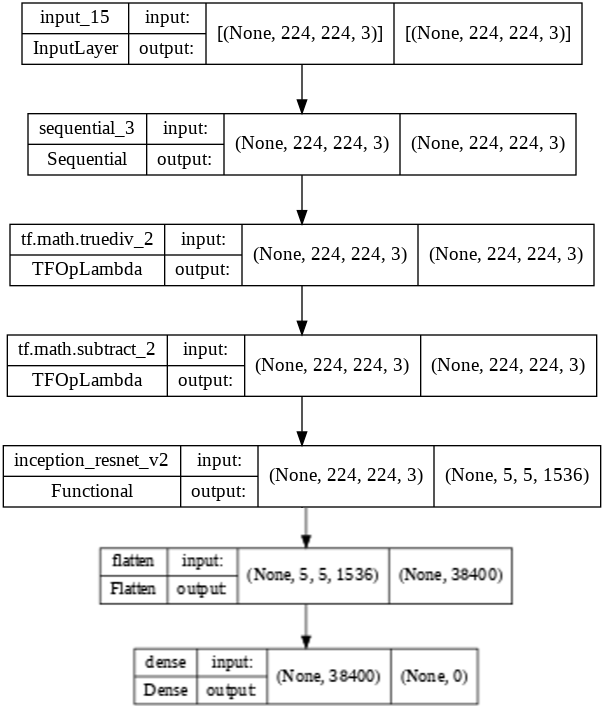
\includegraphics[width=\textwidth]{M4arc.png}
\caption{ Architecture For Inception Resnet V2 model}
\label{fig:Frozen}
\end{figure}
\subsection{Datasets}
The Weed Detection datasets in Soybean Crop consists of a total of 15336 segmented images, with 3249 of soil, 7376 of soybean, 3520 grass and 1191 of broadleaf category of weeds. Each image in the dataset has a pixel size of around 200x180. We split the dataset into 8:2 training and testing images. We use augmentation techniques to increase variability as well as the number of images.  

\subsection{Data Augmentation}
For data augmentation we used already available method in Keras API namely ImageDataGenerator with a batch size of 32 and randomly shifted, flipped, and scaled the images to increase our existing dataset. The ImageDataGenerator provides a quick and easy way to perform the task of data augmentation.  The main benefit of keras ImageDataGenerator is that it augments images on the fly when the model is being trained.  The ImageDataGenerator doesnot add new images to the training dataset but it augments all the dataset after each epoch. In our case we have 12268 images in our training dataset, all these images were augmented after each epoch, therefore in our training process for 10 epoch we trained our model on 12268 original images and $12268\times10$ augmented images.

\subsection{Performance Measures}
The four categories’ labels were converted to one hot vector and probabilistic categorical cross entropy is used as our performance metric. The categorical cross entropy loss computes the loss between true and predicted labels. We implemented early stopping to limit training of our model at an appropriate time by monitoring the improvement in the validation loss metric. 



\section{Experimental Results}
\label{sec:M4-results}
We fitted our model as described in the previous section. We froze all the layers except the initial input layer, we added one dense layer with 4 neurons to categorically classify the four distinct categories. After freezing the weight, we obtained training accuracy of around 0.97 and validation accuracy of 0.97. Similarly, we achieve a training loss as low as 0.38 and validation loss as low as 0.32. Figures \ref{fig:v2fr} and \ref{fig:lossV2} are the learning curves with weight freezing. The validation curve clearly shows that the model is poorly fitted. With this performance, again we hypothesize that unfreezing all the layers of InceptionResNetV2 model  and fine-tuning the weights with our dataset might lead to a better performance. 
\begin{figure}[H]
\centering
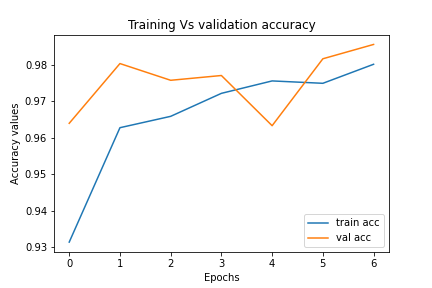
\includegraphics[width=\textwidth]{AccVal_FreezeInceptionResNetV2.png}
\caption{Accuracy curve for InceptionResNetV2 model with weights frozen}
\label{fig:v2fr}
\end{figure}
\begin{figure}[H]
\centering
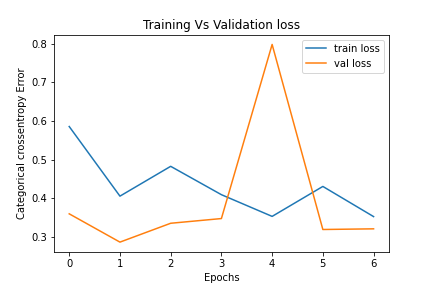
\includegraphics[width=\textwidth]{LossVal_FreezeInceptionResNetV2.png}
\caption{Loss curve for InceptionResNetV2 model with weight frozen}
\label{fig:lossV2}
\end{figure}

\begin{figure}[H]
\centering
\includegraphics[width=\textwidth]{FreezingWeights.png}
\caption{Confusion matrix with freezing of weights}
\label{fig:CM2}
\end{figure}
\begin{tabular}[H]{ | p{3cm}||p{2cm}||p{2cm}||p{2cm}||p{2cm}|}
\hline
 \multicolumn{5}{|c|}{ Table 3.1 :Metrics for Freezing weights during training}\\
 \hline
 Serial Number & Precision & Recall & F1-Score & Support\\
 \hline
 0 - Grass & 0.99 & 0.98 & 0.98 & 350 \\
 1 - Soil & 0.98 & 0.98 & 0.98 & 324\\
 2 - Soybean & 0.99 & 0.99 & 0.99 & 733\\
 3 - Weeds & 0.94 & 0.97 & 0.95 & 120 \\
 Accuracy &  &  & 0.99 & 1527\\
 Macro Average & 0.98 & 0.98 & 0.98 & 1527\\
 Weighted Average & 0.99 & 0.99 & 0.95 & 1527\\
 \hline
\end{tabular}


\vspace{1cm}
The figures \ref{fig:Unfroozen1} and \ref{fig:Unfroozen2} show the learning curves for the fine-tuned fitting approach. With fine tuning we achieve a training accuracy as high as 0.98 and validation accuracy as high as 0.99. Similarly, we obtained training loss to zero and for validation loss even though it shows drastic fluctuation in loss values, finally it reaches to zero. 






Furthermore, the confusion matrix in figure \ref{fig:CM2} shows the true level and predicted levels. Also, table 3.1 shows various metrics of performance.  We can see that the model very rarely being confused between four categories. 




\hfill


\begin{figure}[H]
\centering
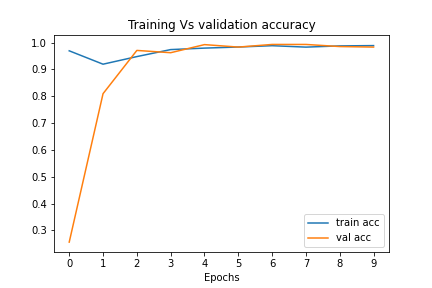
\includegraphics[width=\textwidth]{AccVal_FineTuneInceptionResNetV2.png}
\caption{Accuracy curve for InceptionResNetV2 model with fine-tuning}
\label{fig:Unfroozen1}
\end{figure}

\begin{figure}[H]
\centering
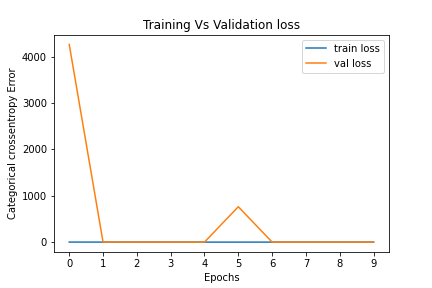
\includegraphics[width=\textwidth]{LossVal_FineTuneInceptionResNetV2.png}
\caption{ Loss curve for InceptionResNetV2 model with fine-tuning}
\label{fig:Unfroozen2}
\end{figure}



\begin{figure}[H]
\centering
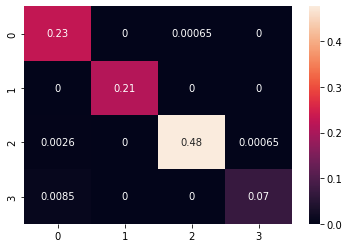
\includegraphics[width=\textwidth]{CFinetuning.png}
\caption{Confusion Matrix with fine-tuning}
\label{fig:CM}
\end{figure}

\hfill

\begin{tabular}[H]{ | p{3cm}||p{2cm}||p{2cm}||p{2cm}||p{2cm}|}
\hline
 \multicolumn{5}{|c|}{ Table 3.1 :Metrics for Fine Tuning weights during training}\\
 \hline
 Serial Number & Precision & Recall & F1-Score & Support\\
 \hline
 0 - Grass & 0.95 & 1.00 & 0.97 & 350 \\
 1 - Soil & 1.00 & 1.00 & 1.00 & 324\\
 2 - Soybean & 1.00 & 0.99 & 1.00 & 733\\
 3 - Weeds & 0.99 & 0.89 & 0.94 & 120 \\
 Accuracy &  &  & 0.99 & 1527\\
 Macro Average & 0.99 & 0.97 & 0.98 & 1527\\
 Weighted Average & 0.99 & 0.99 & 0.99 & 1527\\
 \hline

\end{tabular}

\section{Discussion}

Reviewing the literature, use of residual networks was a step taken in the right
direction. However, the results we got were not aligned to what we thought. We initially froze the base network weights and quickly found that it was
a dead-end with no gradual improvement in the model performance. For this milestone, we implemented a convolutional neural architecture that builds on the inception family of architectures but incorporates residual connections, InceptionResNetV2. Since Inception networks tend to be very deep, it is natural to replace the filter concatenation stage of the Inception
architecture with residual connections. This would allow
Inception to reap all the benefits of the residual approach
while retaining its computational efficiency  \cite{szegedy2017inception} and it leads to getting good results for further classification tasks. We got a better performing model with training efficiency of more than 98\% with patience parameter of 5.

\section{Conclusion}
Till now, we observed that transfer training is one of the right approaches that we could use to train a deep learning model with a smaller dataset. We used a pretrained ResNet50 model already trained on ImageNet dataset for our project. All the results, such as the learning curves, showed some benefit of fine-tuning but the results were not promising as expected. So, we worked on InceptionResNetV2 implementation that makes improvement to ResNet50 architecture with introduction of inception block that leads to a wider network and also being computationally efficient. This approach was significantly better and led to good results. For future work, we will try to run this architecture with more data augmentation and analyse how the performance will vary.

\begin{table}[H]
    \caption{Contributions by team member for Milestone~4.}
    \centering
    \begin{tabular}{|c|c|} \hline
    {\bf Team Member}     &  {\bf Contribution}  \\ \hline
    Shubham Bery     &  Model deployment and report writing  \\
    Shiva Paudel   &  Model deployment and report writing \\
    Puranjit Singh &   Model development and deployment \\
    Kantilata Thapa & Model deployment and report writing \\ \hline
    
    \end{tabular}
    \label{tab:contribution4}
\end{table}

\iffalse
\chapter{Milestone 5: Final Report}


\section{Introduction}
\label{sec:M5-intro}

Remind the reader of the problem you're working on, and what your approach is.  Briefly summarize what your final results are.

Also, remember to update your abstract when you've completed this chapter.

\section{Experimental Setup}
\label{sec:M3-setup}

Describe the setup of your experiments  in sufficient detail for the reader to reproduce them.  Include data sources, preprocessing used, architectures/other approaches used, hyper-parameter values used, performance measures used, other relevant items (e.g., cross-validation).

\section{Experimental Results}
\label{sec:M5-results}

Present your results  using tables, figures, confusion matrices, etc.\ (whatever is appropriate). 

\section{Discussion}

Discuss your experimental results, drawing conclusions that are supported by your experimental results of Section~\ref{sec:M5-results}.   Be careful to not draw conclusions that are not supported by the evidence you present!

\section{Conclusion}

Sum up, including your a summary of your results  (recapitulating that from Section~\ref{sec:M5-intro}).  Also, describe possible avenues for future work (should one continue the project) and list any questions that you have for the instructor and TA regarding your project work.

\textcolor{red}{Remember to cite sources using BiBTeX and add those references to the end of this document!}

It is okay to cite some websites and tutorials (if you first look up how to properly cite them!), but you must also cite some refereed publications from conferences and/or journals.

Finally, in Table~\ref{tab:contribution5}, list each member of your team with a brief summary of that member's contribution to this milestone.

\begin{table}[]
    \caption{Contributions by team member for Milestone~5.}
    \centering
    \begin{tabular}{|c|c|} \hline
    {\bf Team Member}     &  {\bf Contribution}  \\ \hline
    Member1     &  Contribution1 \\
    Member2     &  Contribution2 \\
    Member3     &  Contribution3 \\ \hline
    \end{tabular}
    \label{tab:contribution5}
\end{table}

\appendix

\chapter{First Appendix}

An appendix is used only if necessary (remove this chapter if you don't use one). It contains supplementary materials/extra details such as extensive experimental results (e.g., hyper-parameter search results, where the most interesting ones are in the main text and the rest are dumped here), detailed proofs, etc. 

Create as many appendices as needed by adding chapters. All such chapters must be before the bibliography. 
\fi

\bibliographystyle{plainurl}
\bibliography{main}

\end{document}
